% preset
\documentclass[a4paper, 12pt]{article}\usepackage[dvipdfmx]{graphicx}\usepackage[]{xcolor}
% maxwidth is the original width if it is less than linewidth
% otherwise use linewidth (to make sure the graphics do not exceed the margin)
\makeatletter
\def\maxwidth{ %
  \ifdim\Gin@nat@width>\linewidth
    \linewidth
  \else
    \Gin@nat@width
  \fi
}
\makeatother

\definecolor{fgcolor}{rgb}{0.345, 0.345, 0.345}
\newcommand{\hlnum}[1]{\textcolor[rgb]{0.686,0.059,0.569}{#1}}%
\newcommand{\hlstr}[1]{\textcolor[rgb]{0.192,0.494,0.8}{#1}}%
\newcommand{\hlcom}[1]{\textcolor[rgb]{0.678,0.584,0.686}{\textit{#1}}}%
\newcommand{\hlopt}[1]{\textcolor[rgb]{0,0,0}{#1}}%
\newcommand{\hlstd}[1]{\textcolor[rgb]{0.345,0.345,0.345}{#1}}%
\newcommand{\hlkwa}[1]{\textcolor[rgb]{0.161,0.373,0.58}{\textbf{#1}}}%
\newcommand{\hlkwb}[1]{\textcolor[rgb]{0.69,0.353,0.396}{#1}}%
\newcommand{\hlkwc}[1]{\textcolor[rgb]{0.333,0.667,0.333}{#1}}%
\newcommand{\hlkwd}[1]{\textcolor[rgb]{0.737,0.353,0.396}{\textbf{#1}}}%
\let\hlipl\hlkwb

\usepackage{framed}
\makeatletter
\newenvironment{kframe}{%
 \def\at@end@of@kframe{}%
 \ifinner\ifhmode%
  \def\at@end@of@kframe{\end{minipage}}%
  \begin{minipage}{\columnwidth}%
 \fi\fi%
 \def\FrameCommand##1{\hskip\@totalleftmargin \hskip-\fboxsep
 \colorbox{shadecolor}{##1}\hskip-\fboxsep
     % There is no \\@totalrightmargin, so:
     \hskip-\linewidth \hskip-\@totalleftmargin \hskip\columnwidth}%
 \MakeFramed {\advance\hsize-\width
   \@totalleftmargin\z@ \linewidth\hsize
   \@setminipage}}%
 {\par\unskip\endMakeFramed%
 \at@end@of@kframe}
\makeatother

\definecolor{shadecolor}{rgb}{.97, .97, .97}
\definecolor{messagecolor}{rgb}{0, 0, 0}
\definecolor{warningcolor}{rgb}{1, 0, 1}
\definecolor{errorcolor}{rgb}{1, 0, 0}
\newenvironment{knitrout}{}{} % an empty environment to be redefined in TeX

\usepackage{alltt}
\title{Age might not matter - an observational study of the voter discount of young candidates}
\author{Dai Sasaki}
\date{Last update: 21 May 2023}

% packages
\usepackage[utf8]{inputenc}
\usepackage{amsmath}
\usepackage{amsfonts}
\usepackage{array}
\usepackage{booktabs}
\usepackage{colortbl}
\usepackage{dcolumn}
\usepackage{float}
\usepackage{geometry}
\usepackage[dvipdfmx]{graphicx}
\usepackage{hyperref}
\usepackage{multirow}
\usepackage{natbib}
\usepackage[normalem]{ulem}
\usepackage{ntheorem}
\usepackage{pdflscape}
\usepackage{rotating}
\usepackage{setspace}
\usepackage{subfigure}
\usepackage{tabularx}
\usepackage{threeparttable}
\usepackage{wrapfig}
\usepackage{xcolor}

% page styling
\geometry{
  a4paper,
  left=28mm,
  right=28mm,
  bottom=3cm,
  top=3cm}
\pagestyle{plain}
\pagenumbering{arabic}
\linespread{2.0}

% command definition
\newlength{\spacebox}
\settowidth{\spacebox}{012345678901}
\newcommand{\sepspace}{\vspace*{2em}}
\newcommand{\sepspacesmall}{\vspace*{0.3em}}
\theoremseparator{:}
\newtheorem{hyp}{Hypothesis}

% begin document
\IfFileExists{upquote.sty}{\usepackage{upquote}}{}
\begin{document}

\maketitle

\begin{abstract}
Despite accounting for a certain proportion of the population, the youth in Japan are under-represented in parliament. One possible explanation for the lack of young parliamentarians is that voters might punish them for being young, while this intuitive explanation has been repudiated in the literature that employs experimental methods. This paper serves to further ratify the empirical evidence. It introduces an observational study on the relationship between candidates age and their electoral performance in Japan, using a dataset containing the information of all post-WW2 candidates that ran for the Japanese lower house election. Consistent with the preceding findings, we find no evidence of voter discrimination of younger candidates. The evidence suggests that in order to find out potential causes of the youth under-representation, we should focus more on the upper stream of the electoral process.
\end{abstract}

\newpage

\tableofcontents

\newpage

% Ch.1
\section{Introduction} \label{ch1}

The youth in Japan account for a particular part of the population. However, they are somehow under-represented in the arena of political decision-making. For example, let the threshold of being "young" be 40, and we find that "young politicians" account only for about 3.4 \% in the Japanese lower house \citep{shugiin2023}, while there are about 40 \% of "young people" in its whole population \citep*{mhlw2021}. Considering the minimum age of eligibility (25 years old for the lower house), the youth are under-represented in parliament to a considerable extent. 

Although the reasons for youth under-representation in Japan are unclear and might not be specified, there is one possible explanation: voters might punish young candidates for their age. In other words, voters might choose not to vote for young candidates, perhaps because they consider them immature, inexperienced, or inferior to their older counterparts. 

Although not always directly, this hypothesis has been tested and repudiated in the political science literature. Researchers have relied on conjoint survey experiments to see voters' preferences for candidates' attributes, specifically how voters evaluate candidates' age (e.g., \citet{horiuchi2020identifying, mcclean2022too, eshima2022just}). The research found no evidence that voters prefer older candidates to younger counterparts or discriminate against young candidates; in fact, voters in those experiments disliked elderly candidates and favored younger ones. 

This paper uses observational data to provide alternative evidence to this question from a different perspective. With profiles of all the candidates who ran for the Japanese lower house election from 1994 to 2020, I conducted quantitative analyses to explore the relationship between candidates' age and vote share in the Japanese lower house election. Most importantly, they suggest that voters should not be blamed for the current youth under-representation in the Japanese parliament. In other words, while data apparently show that voters discount younger candidates for their age, a closer look reveals that voters might respond to other attributes correlated with candidates' age, such as incumbency status, electoral expenditure, and political dynasty. 

The contribution of this paper is threefold. Firstly, it provides a candidate-level analysis in the context of age representation. Until recently, there had been only a tiny amount of attention to the youth's under-representation. In addition, the few works exploring factors that affect the presence of young politicians in parliament focus on country-level differences, i.e., institutions (e.g., \citet{joshi2013representation}) \footnotemark{}, thus not discerning micro-level factors that control young candidates' entrance into the political arena of decision making. In contrast, this paper analyses candidate-level data and points, although not causally, to the potential factors that hinder young candidates from well-represented. 

\footnotetext{\citet{joshi2013representation} finds support for the theory that proportional electoral systems (``PR" hereafter) tend to favor younger candidates, compared to single member district plurality electoral systems (``SMDP" hereafter). Rationales behind this are threefold: firstly, as incumbency advantage is more strongly pronounced in single-member districts than in other electoral systems, neither younger candidates, who tend to be non-incumbent, are likely to obtain a large amount of votes, nor do they get a nomination from their party. Secondly, while PR systems induce party-centered politics, SMDP systems lead to candidate-centered politics, benefiting older candidates with larger electoral resources. Thirdly, parties have a larger incentive to let younger candidates gain experience by placing them in their party list.}

Secondly, this paper exploits a different form of data and produces evidence that further consolidates the existing literature—previous research employed survey experiments to renounce the possibility of voter discrimination against young candidates. With the aid of observational data, this paper serves to ratify the absence of voter-level contribution to youth under-representation in Japan. 

Thirdly, this paper sheds light on factors in work behind the spurious correlation between candidates' age and their likelihood of winning the election. Analyses in the paper suggest that the correlation between the two is, at best, superficial and posit that candidates' other attributes, such as the financial scale of their campaign, their party affiliation, and their political dynasty, are responsible for that relationship. This finding shifts our attention upstream to the candidate selection process, whether as individuals or in political parties and further to the pool of potential candidates, just as in the female representation literature \citep{lawless2010still}. 

This paper progresses as follows. It first describes how and to what extent the youth is under-represented in the Japanese parliament. By graphically comparing age distributions of the Japanese population, its lower house candidates, and lower house parliamentarians, it reveals that there are neither as many young candidates nor MPs as young citizens. It next explores the existing literature. It includes reviews on the concept of representation, how it relates to the representation of the youth, and what researchers have found on the youth representation in Japan. Then, after introducing data, models, and methods employed, I present quantitative analyses of the relationship between candidates' age and their vote share in Japanese lower house elections. Using data covering all Japanese lower house candidates between 1994 and 2020, I conduct multiple regressions of candidates' age on their vote shares. While simple, univariate models imply voter discrimination of young candidates, this result is overturned by more elaborate models that include interaction terms and consider heterogeneity among different elections and locations. I further conduct an additional analysis that employs matching, whose result is in line with the paper's main findings. The last part of the paper discusses the implications of its results. Mentioning the paper's contributions and drawbacks, this final part also accounts for the future direction the literature could extend. 

% Ch.2
\section{Youth under-representation in Japan} \label{ch2}

This chapter reviews how and to what extent the youth are under-represented in the Japanese parliament, particularly in the lower house. Specifically, it compares the age composition of politicians and to-be politicians, the population, and its sub-groups. This contrast reveals two things: firstly, few young candidates, let alone young parliamentarians, are in the Japanese lower house. Not only do young people enter parliament less than those of other generations, they do not run as much for the election. Secondly, we also see that young candidates have less likelihood to win the election than those of middle or older age. While there are already few of them when they run for the election, they are somehow more likely to eliminated in the competition than those of other age groups. These implications lead to another question: does age itself matter to win the election?

\subsection{The lack of young politicians} \label{ch2.1}

How and to what extent are young people under-represented in parliament? We could look at the age composition of MPs and the population. Figure \ref{mp} compares the age distributions of MPs in the Japanese lower house and the population in 2021 \footnotemark{}. Two histograms in the figure have vastly different shapes. While the population is distributed somewhat flatly and bimodally, the MPs' age has a condensed distribution with its single, eminent mode around 60 years old and its short tails \footnotemark{}. Overall, we can see that the middle-aged population is over-represented, while young people in their thirties or younger and the elderly in their late seventies or older are under-represented. 

\footnotetext{The youngest and oldest MPs as of November 2022 are each 31 and 84 years old.}

\begin{figure}
\centering
  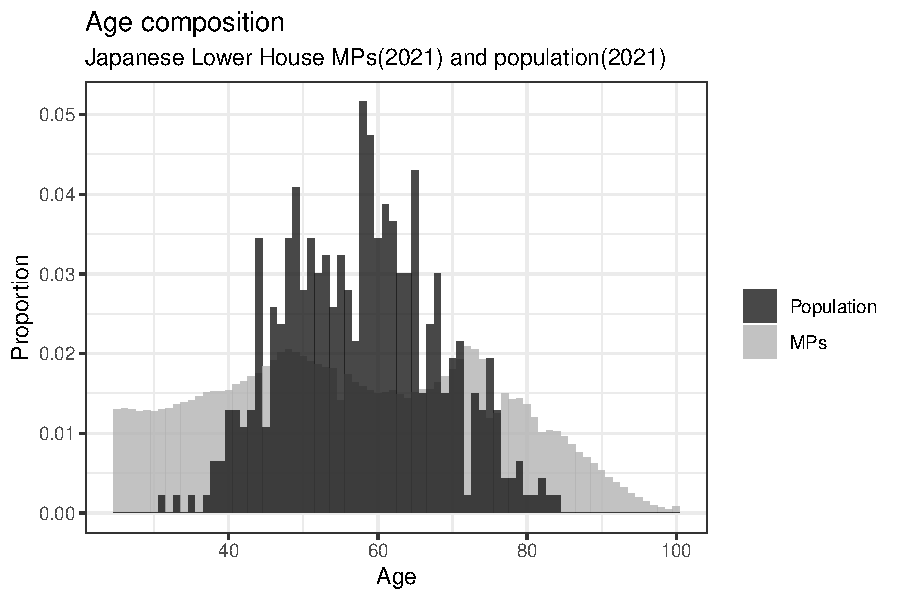
\includegraphics[width=0.8\textwidth]{figure/comp_age/comp_mp.pdf}
  \caption{Age composition: Lower house MPs and population}
  \label{mp}
\end{figure}
\footnotetext{MPs data are taken from the Japanese lower house website \citep{shugiin}. Demographic data are based on demographic statistics created by the Ministry of Health, Labour and Welfare\citep{mhlw2021}.}

\subsection{The lack of young candidates}

The focus in this subsection moves upstream toward the election. Next, I compare the Japanese lower house candidates and the country's population. They demonstrate that youth under-representation exists even before candidates enter parliament. First of all, figure \ref{allAge} contrasts the age composition of candidates in the 2014 election and the population in 2021 \footnotemark{}. The x-axis and y-axis each represent candidates' age and the proportion of candidates of a certain age. The length of each tail differs a lot. Compared to the population, the distribution of candidates has shorter upper and lower tails. The youngest and oldest candidates are 25 and 86 years old. Note that candidates ranging from 0 to 25 years old are truncated due to the minimum eligible age to run for the lower house. 

% allAge
\begin{figure}
\centering
  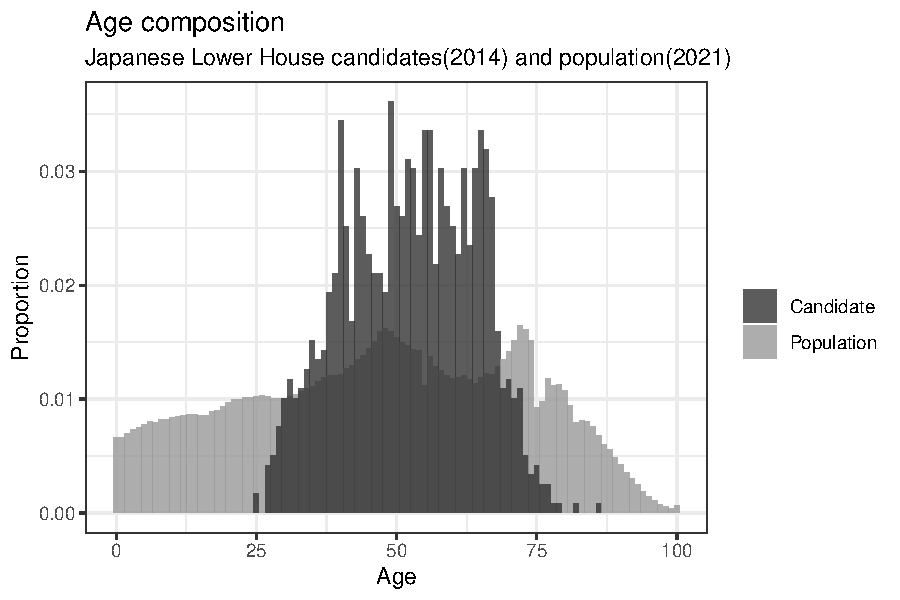
\includegraphics[width=0.8\textwidth]{figure/comp_age/comp_all.pdf}
  \caption{Age composition: Lower house candidates and population}
  \label{allAge}
\end{figure}
% footnote for allAge
\footnotetext{Data of candidates' age are based on the Reed-Smith Japanese House of Representatives Elections Dataset\citep{reedsmith2018}.}

What if we focus on the population eligible to run? Figure \ref{o25} compares the age composition of the candidates and the population similarly as in figure \ref{allAge}, while focusing on people older than 25 \footnotemark{}. Although the imbalance between the two groups is smaller than in the previous figure, we can still see some gaps. For example, the heights of red and blue bars in the range from 25 to 40 years old are noticeably different. We also notice that people in their forties to sixties are vastly over-represented. In sum, these comparisons display the lack of young candidates. Indeed, there are few young politicians in parliament. However, it might not necessarily be the election responsible for that under-representation. Young politicians are missing, and even at the candidate stage, young to-be politicians are absent.

\begin{figure}
\centering
  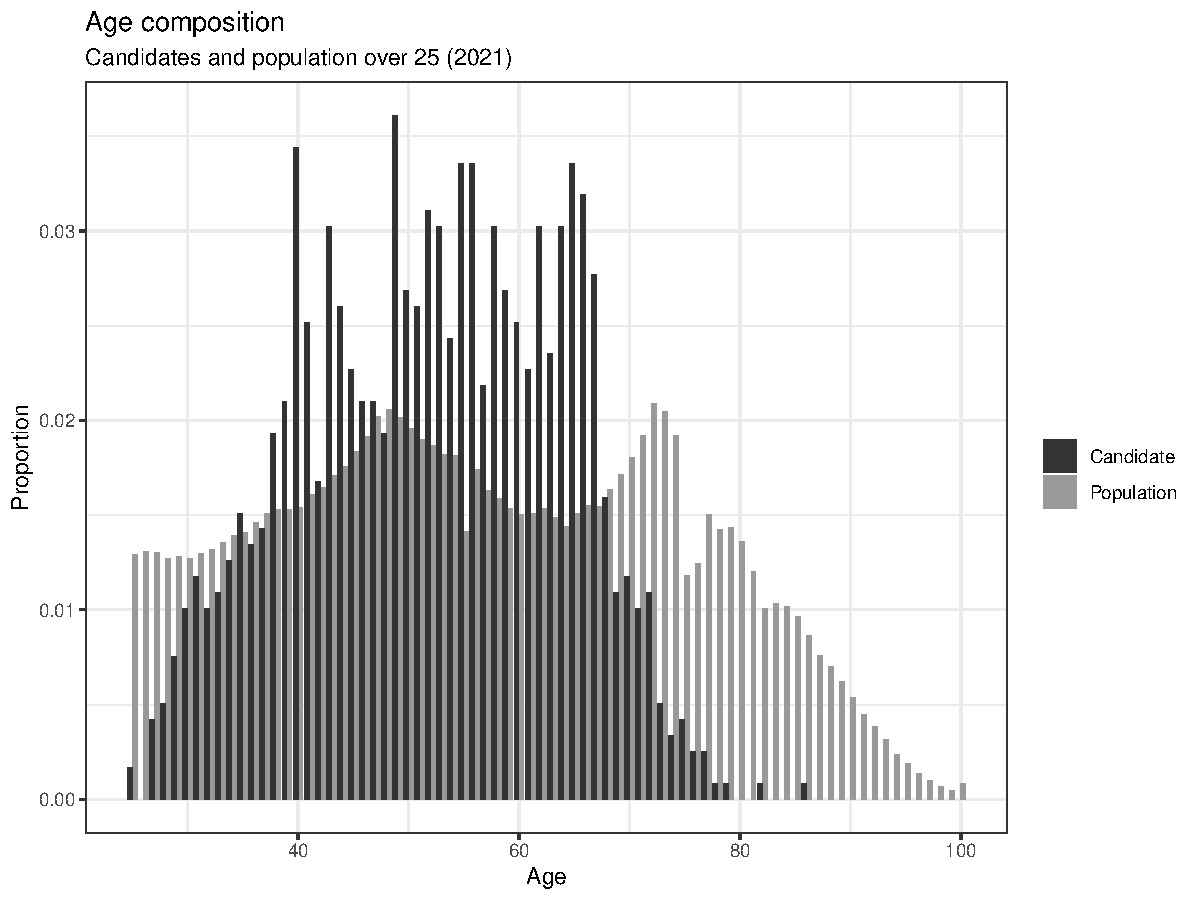
\includegraphics[width=0.8\textwidth]{figure/comp_age/comp_o25.pdf}
  \caption{Age composition: Lower house candidates and population over 25}
  \label{o25}
\end{figure}
\footnotetext{For the population, the y-axis represents the proportion that people of certain age account for in the population over 25.}

\subsection{The lack of young winners} \label{ch2.2}

The previous section clarified that young people are already under-represented in the pool of candidates. Does it mean that the representation levels of that population group are not different between candidates and winners? Figure \ref{winners} might answer that question. The figure features two histograms. On the left-hand side is a comparison of age composition among 1. population eligible to vote (i.e., over 20 years old), 2. candidates, and 3. winners. On the right-hand side is its slightly modified version, presenting the population eligible to run (i.e., over 25 years old). Red bars denote candidates, blue winners, and green populations in both histograms. An instant look would suffice to see a similar tendency in the previous figures. As does the distribution of candidates, that of electoral winners has shorter tails and a higher mode. However, more importantly, a detailed scrutiny reveals the different heights of red and blue bars: while the blue bars are mostly taller than the red bars in the range from 40 to 85, that relationship is reversed for younger ages. That is, those under 40 comprise a minor part of the electoral winners than they do of the candidates. In other words, young candidates are likelier than other age groups to be eliminated in the electoral race. Therefore, the answer to the question above is no: while young people are under-represented in the pool of candidates and winners, the level of under-representation is more severe for the latter. 

\begin{figure}[h]
\centering
  \subfigure{{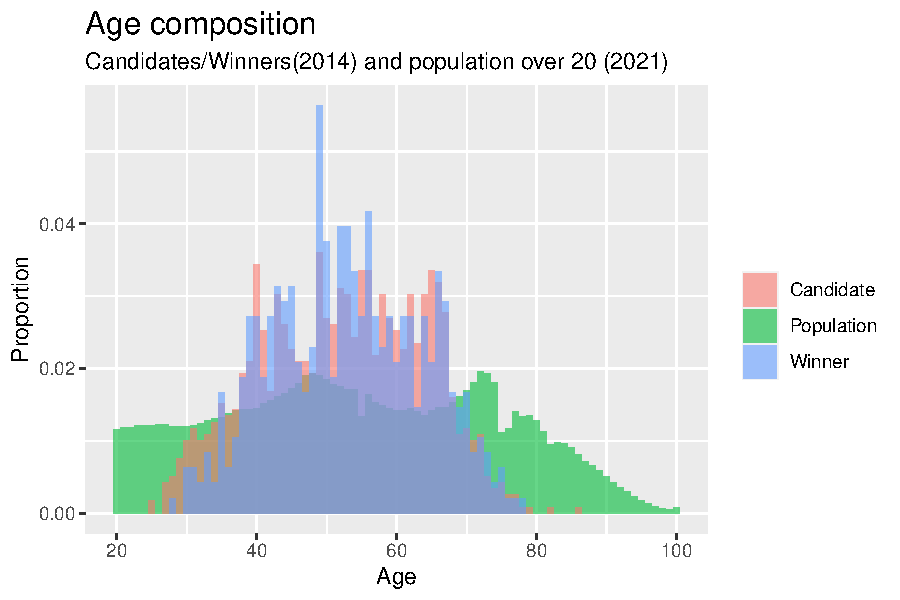
\includegraphics[width=0.48\textwidth]{figure/comp_age/comp_o20.pdf}}}
  \hfill
  \subfigure{{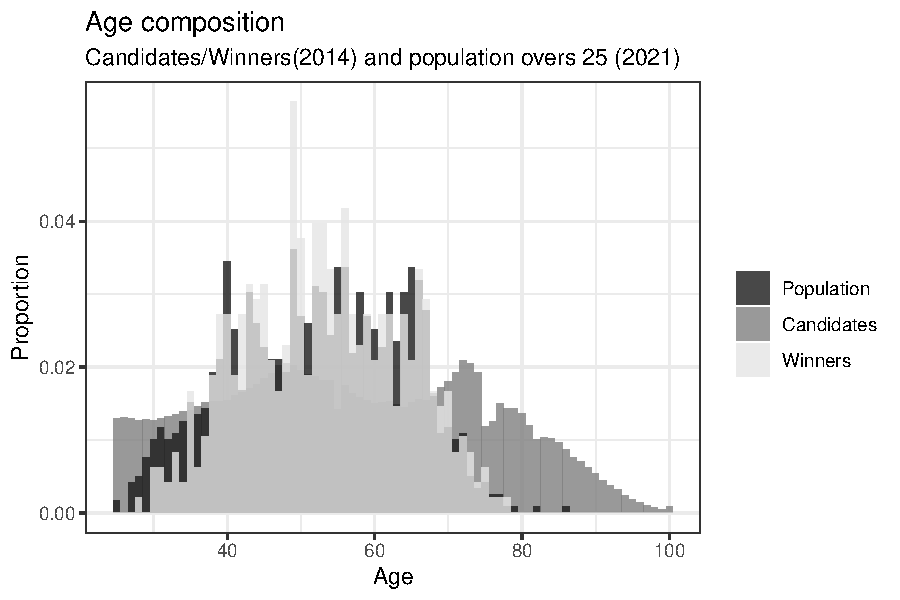
\includegraphics[width = 0.48\textwidth]{figure/comp_age/comp_o25w.pdf}}}
  \caption{Age composition: candidates, winners, and population}
  \label{winners}
\end{figure}

This section has seen how the youth are under-represented in the Japanese parliament. It points to two things: First, youth under-representation exists before and after the election. In other words, the age imbalance in the Diet might not only be due to the electoral system; young people are already under-represented at the start line when they run for the election. 

Still, it is neither that the election is not crucial nor that candidates' age does not matter in the election. A closer look into the data reveals that the few young candidates running for the election might be more likely to be defeated than those of the other age groups. 

This finding stimulates the key research question in this paper: does age in itself matter in the election? In other words, are young candidates punished by voters solely for their age? It could seemingly be true that young candidates have to struggle in adverse circumstances, but it could be either because voters discriminate against young politicians or because voters evaluate those in other age groups with more experience. Alternatively, voters might support candidates from specific political parties, and those specific parties happen to choose candidates of the middle ages. Furthermore, it could be that candidates with advanced careers have a sizeable electoral budget than their young counterparts do. 

The rest of this paper seeks to answer this question. The next chapter reviews the literature and proposes hypotheses to be tested in the following parts. 

% Ch.3
\section{Literature review and hypothesis} \label{ch3}

To propose some hypotheses, this chapter reviews the existing literature on relevant themes and topics, such as representation, youth descriptive representation, and youth representation in Japan. This paper addresses the research question: "Does candidates' age matter in the election?". This question derives from extensive research in the representation literature, including works on minorities or other under-represented groups, such as ethnic or racial minorities and women. 

This chapter first describes how researchers defined and elaborated their understandings of representation and why they did that. The second section handles the representation of a specific group of people, the youth. Youth representation has a common ground with representation of other groups. This section illustrates how researchers saw this connection and how they exploited it to deliver findings that spark this paper's interest. 

The third section treats how existing research has analyzed youth representation in Japan and presents the hypotheses on the "age effect" on candidates' performance in the election. As the previous chapter showed, young people are under-represented in the pre and post-election stages. In response to this unbalanced situation and concerns of its potential consequences, recent years have seen researchers advance in this area, on which this paper and its argument are based. This paper contributes in three ways: preceding works have worked on these topics either 1. in experimental situations or 2. in the context of other countries. This paper tackles the same topic with the aim of 1. providing evidence based on real-world circumstances, 2. in Japan; thus, 3. shedding light on factors in work behind the spurious correlation between candidates' age and their likelihood of winning the election. 

\subsection{Representation} \label{ch3.1}

What is representation? According to Pitkin, its definition is multifaceted. She mentioned four types of representation \citep{pitkin1967concept}: firstly, formalistic representation refers to formal mechanisms and institutions that precede and enable it. When someone is formally represented, he or she is authorized to act on behalf of the represented (\citet{pitkin1967concept}, 38-39). 
% symbolic
Secondly, there is a symbolic representation, which resembles the role of a national flag: it represents the nation, which is, in fact, not present (\citet{pitkin1967concept}, 92). A real example in the context of Japan is the emperor, whom the constitution of Japan declares to be "the symbol of the State and of the unity of the People, deriving his position from the will of the people with whom resides sovereign power" (\citet{jpconst}, Article 1, Chapter 1). 
% descriptive
The third type of representation, the most relevant type to this paper, is descriptive representation. It refers to the making of something formerly absent by resemblance: to represent something descriptively means to stand for the represented in as unblemished a way as possible (\citet{pitkin1967concept}, 60). 

% substantive
Unlike the three types of representation mentioned so far, the last type of representation, substantive representation, focuses on the aspect of an activity. This view of the concept allows the existence of representatives as "agent or actor for others" and validates the discussion of what they ought to do (\citet{pitkin1967concept}, 115). 

% finishing off weak...
Descriptive representation has attracted the scholarly attention of political scientists, especially those studying American politics, in which disadvantaged groups' representation has been a constant topic of academic debate (e.g., \citet{mansbridge1999should, lemi2022descriptive}). This is relevant to the presumption that the notion of descriptive representation entails the idea that representative bodies be a "mirror" of the represented \citep{pitkin1967concept}. In this regard, an argument holds that certain groups of people be represented by descriptive representatives, individuals who share common characteristics, backgrounds, and experiences with those groups. In real-life politics, different groups of constituents have different sets of values to be represented in the governing bodies. However, who represents or should represent the interests of minorities or under-represented groups, such as ethnic or racial minorities and women? Academics have worked on this question, both normatively and empirically. 

% on subRep and modern poliSci, in conjunction with descriptive representation
Substantive representation is also a target of scrutiny by political scientists, as descriptive representation might not solely represent a group's interests. In Pitkin's words, descriptive representatives do not necessarily "act for" the represented. This link between two forms of representation has drawn an enormous amount of scholarly attention, and researchers have not agreed on the existence of this connection (e.g., \citet{mansbridge1999should, espirito2020does, wangnerud2009women}). For example, \citet{mansbridge1999should} writes in the context of blacks and women's representation: "Descriptive representation is not popular among normative theorists... Empirical political scientists studying women and Black legislators have had similar negative assessments" (3), while she herself argues for this relationship in the same article, claiming that descriptive representation helps enhance substantive representation by making their "uncrystallized interests" tangible(1). 

One of the significant difficulties when discussing substantive representation is its multifaceted nature. Again in Pitking's words, substantive representation is about the action to represent. It could naturally imply more than a single type of activity. For example, more recent studies find a positive relationship between women's descriptive representation in national parliaments and their level of civic engagement \citep{norris2009one}, while indicating no effect of legislator's age on their representational behavior \citep{tam2022does}. Substantive representation encompasses multiple dimensions of representational actions, and we have not yet fully reached its connection with descriptive representation. 

Another vital question rests unanswered: why is representation worth researching? One of the most persuasive answers is that it is closely tied to a core value deemed essential in a democracy. A strand of theories on democracy views representation this way. In Roald Dahl's classic work on the essence of democracy, he claimed that an ideal form of democracy, which he called "polyarchy," guarantees the following eight qualities through its institutions: freedom to form and join organizations, freedom of expression, suffrage, politicians' right to compete for popular support, alternative source of information, eligibility to public offices, free and fair elections, and institutions to warrant government's accountability \citep{dahl2008polyarchy}. Further, he discussed that these eight requirements constitute two dimensions foundational to democracy: contestation and inclusion \citep{dahl2008polyarchy, coppedge2008two}. Of those two, the former indicates "the extent of permissible opposition, public contestation, or political competition", while the latter refers to "the breadth of the right to participate in public contestation" (\citet{dahl2008polyarchy}, 4). In other words, Dahl esteemed it indispensable for the ideal democracy to entitle a wide range of people to the right and opportunities to express their opposition, to contest power openly, or to be involved in the election and other forms of political competition. 

\subsection{Youth representation} \label{ch3.2}

% why
How do the theory of and findings on representation apply to the youth? As the previous chapter suggested, the youth are under-represented in parliament (for other examples, see \citet{joshi2013representation, mcclean2020thesis, stockemer2023young}). However, this fact itself does not necessitate the youth receiving representation in parliament. First of all, why should the youth be represented? 

% life-cycle effect 
Take a step away from the youth, a specific age group, and view people of different age groups more broadly. Generally, take one point in time, and voters of different age groups have different political values. This dissimilarity can be explained as a mixture of two different effects \citep{inglehart2008changing, dimock2019defining, webster2019older}. Firstly, the life-cycle effect shifts a person's values, attitudes, and behaviors as he or she ages (e.g., \citet{plutzer2002becoming}). Aging involves changes in one's life stage and changes in one's living environment. For example, a teenager who lived with his or her parents might go on to university and start to live alone. This person could later marry and have children, forming his or her own family. The kids would eventually move out of the house. People could experience all those life-stage changes as they get old, and each of those changes would make them respond to their surroundings differently. Political values are among what pass together with age. People might become more aware of healthcare-related policies as they become older and more exposed to health-related risks. And just as the elderly worry about their healthcare, the youth could be more responsive to specific issues than people of other age groups. 

% cohort effect
The other effect, the cohort effect, is related to the birth cohort a person belongs to. People in different cohorts grow up in different environments, and this variance in the default settings leads to different political values and ideas. Take two different generations as examples, Millennials and Generation Z \footnotemark{}. Millennials entered the workforce as the large-scale recession started to cause the global economy gloomy prospects. As a result, many of their choices at various life stages were made under the surrounding, unpromising social and economic situations. These cohort effects would shape or bind Millenials' decisions and choices for a long time. For Generation Z, technology has had a vast, unique influence on their surrounding environment \citep{dimock2019defining}. From early times, their surroundings have been filled with connections with someone or something in faraway places. The Internet, mobile devices, and social media enabled them to get to know and keep in touch with their friends on different continents whom they have never seen in person. They also allowed Gen-Zers to keep up with real-time information about what was happening worldwide. Every hour, news feeds on their social media applications tell them about difficulties refugees face, hate crimes against sexual minorities, or wildfires caused by climate change. Gen-Zers come to shape their political stands and policy preferences with all those information. 

\footnotetext{In the definition of Pew research center, one's birth year decides the label of their cohort. For example, Millennials refer to people born between 1981 and 1996. Similarly, anyone born after 1996 belongs to Generation Z \citep{dimock2019defining}.}

% summary of why
In sum, people in different age groups possess different political values and policy preferences due to their current life stages or their surrounding environments that have shaped their day-to-day activities. Young citizens are no exceptions: if we define people under 40 to be "young," they overlap with the sum of Millenials and Generation Z. They tend to possess post-materialist values rather than materialist values \citep{inglehart2008changing}; they are more likely to have different ideas on issues, such as immigration, gender, and environmental problems \citep{dimock2019defining, webster2019older}. Young citizens with distinct perspectives on various policy issues are under-represented in parliament, which could be why they deserve a larger share of representation. 

% how
How is youth representation achieved? A simple answer, parallel to the arguments on other groups' representation, would be to elect more young politicians for parliament. Voters seem to agree with this: it is well-known that voters rely on a variety of heuristics, i.e., easy-to-recognize features of candidates like their party affiliation and gender, in order to decide whom to vote for(\citet{fortunato2019heuristics}. See, for example, \citet{sanbonmatsu2002gender, shugart2005looking, coffe2021candidate}). Candidates' age is one of them. Researchers have found that larger age distances between voters and candidates reduce the probability of voters casting a vote for their co-partisans \citep{sevi2021young}. In a more youth-specific context, young people seem more likely to vote for young candidates \citep{webster2019older}. 

% link to RQ
However, this is about the lowest voter-level relationship between candidates' age and voters' preferences. Questions remain on the higher-level relationship between candidates' age and their consequent performances in the election \footnotemark{}. Different factors enter this layer: connections between age and electoral results could be mediated via the amounts of electoral resources, such as campaign spending and party affiliation. This leads to a research question: "Does age itself matter in the election?" In this regard, the following section summarizes how the literature has worked on this question, especially in the context of Japan, and proposes hypotheses. 

\footnotetext{Also, the relationship between the descriptive and substantive representation of the youth is unclear. While some research finds a causal effect of the former on the latter \citep{mcclean2021does}, there are cases where null effects remain \citep{tam2022does}. General problems of connections between the two might also apply here: substantive representation involves "actions for" the represented that encompasses multiple policy aspects, and we might not necessarily see one-way connections regarding all of those issues. }

\subsection{Youth representation in Japan; Hypothesis} \label{ch3.3}

As the previous chapter showed, the Japanese parliament has quite a small number of young candidates and members, in stark contrast with the proportion of the population that this group of people accounts for. Furthermore, electoral races seem to be more averse toward these few young candidates than toward candidates of other age groups, as the figure \ref{winners} suggests. Perhaps the election stage might be doing some trick behind this situation unfavorable for the youth. 

This paper brings a key research question, "Does age itself matter in the election?" Despite the election working unfavorably toward the youth, we are unsure what matters in that process. Seen from the perspective of young candidates, it could be either because of their age or their lack of career, political resources, or party affiliation. On the voter's side, they might decide not to vote for young candidates because their age reflects inexperience. Instead, they might vote for the incumbent or their co-partisan, and that candidate might happen to be middle-aged or older. 

Scholars have recently employed survey experiments to explore this ``age effect" \citep{horiuchi2020identifying, eshima2022just, mcclean2022too}. These studies employ conjoint experiments, where participants choose one of two hypothetical candidate profiles with several attributes. The order and levels of these attributes are randomized. Findings from this strand of research suggest the absence of this type of age effect: in general, participants do not despise young candidates. On the contrary, the reverse might be true: participants in these experiments consistently disliked older hypothetical candidates \footnotemark{}. Overall, experimental findings are somewhat suggestive of the negative age effect. 

% on Eshima et al.(2022)
\footnotetext{This negative age effect for older candidates could hold even with a slight age difference if voters perceive that difference to be somewhat meaningful. In addition to a meta-analysis of candidate-choice experiments, \citet{eshima2022just} conducts a conjoint experiment where authors compare voter evaluations of candidates aged 69 and 70. They find a significant penalty for the older candidate.}

While the literature has explored the age effect experimentally, little research works on this topic using data from actual candidates. As far as I am concerned, \citet{stockemer2023young} is the only work that shares the research question with this paper which relies on non-hypothetical candidate data, which finds no direct age effect on candidates' performances in the U.S. House of Representatives election and its primary. By using observational data of candidates in the Japanese lower house election, this paper fills the gap in the literature. 

Regarding the age effect in the election, two contradicting hypotheses are possible. Firstly, we could hypothesize that voters prefer older candidates on average. Multiple lines of reasoning are feasible, and they are not mutually exclusive: 

\begin{enumerate}
  \item The age composition of Japanese voters is not constant across generations (See figure \ref{voters}). As voters are generally more likely to vote for candidates more proximate to them in terms of age, the aging electorate might prefer older candidates overall. 
  
  \item Voter faced with multiple choices of candidates, voters might evaluate older candidates as more experienced while disregarding younger candidates as inexperienced. 
\end{enumerate}  

% age composition, voters
\begin{figure}
\centering
  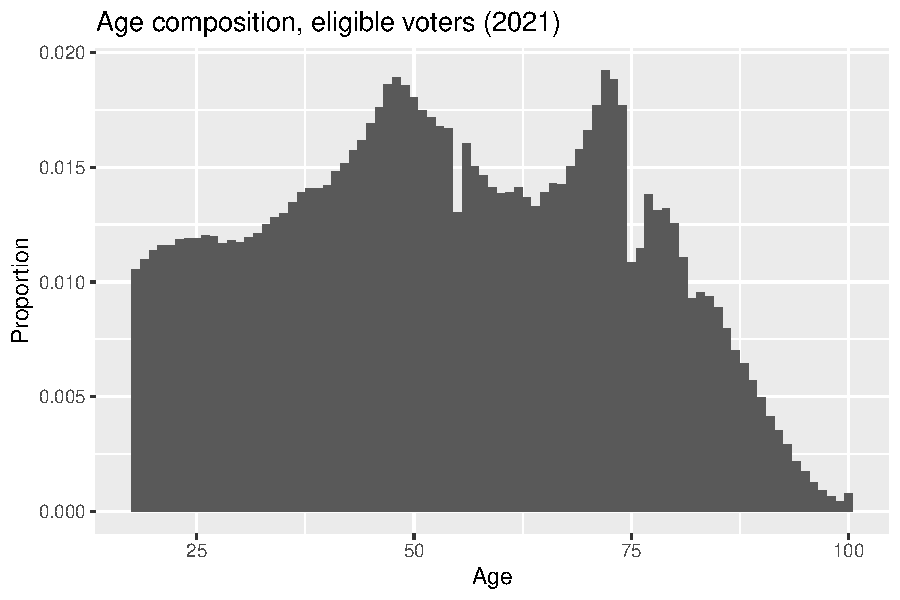
\includegraphics[width=0.8\textwidth]{figure/comp_age/pop_voters.pdf}
  \caption{Age composition: eligible voters}
  \label{voters}
\end{figure}

Thus, while the exact mechanism behind voters' evaluation of candidates' age is beyond this paper's scope, the following hypothesis holds: 

\begin{hyp}[H\ref{hyp:first}] \label{hyp:first}
Younger candidates perform worse than candidates of other ages, all other things equal.
\end{hyp}

The counter hypothesis is also possible: age in itself might not matter. Whereas young candidates tend to perform worse than candidates of other ages, this could be due to confounding factors. For example, young people might 1. be poorer in financial resources, 2. have weaker political backgrounds and supports, or 3. are less likely to be recruited and nominated by strong parties. Thus, 

\begin{hyp}[H\ref{hyp:second}] \label{hyp:second}
Younger candidates perform equally as candidates of other ages, all other things equal.
\end{hyp}

The following chapter describes this paper's data, models, and methods. 

% Ch.4
\section{Data, method, and model} \label{ch4}

This chapter introduces the data, models, and methods used in this paper. This paper contributes to the literature by analyzing observational data of real candidates in the Japanese lower house elections. Although it does not intend to make causal claims about the relationship between candidates' age and their performances in the election, it tries to reduce as much bias as possible via methods available to maintain the reliability of its results. 

This chapter consists of three sections. The first section describes the data set to be used in the empirical analysis. It also discusses the data's strengths and pitfalls and justifies this paper's pre-processing of them. The second section proposes parametric models employed in the analysis. Specifically, it introduces the baseline and additional models, including confounders and fixed effects. The last section first lists the potential problems of the data and methods and then presents some remedies that could reduce them. Namely, this paper turns to multiple imputations to solve the missing data problem and matching as an alternative way of pre-processing the data. While these methods might not solve the problems this paper bears entirely, they could somewhat enhance the validity of its results. 

\subsection{Data} \label{ch4.1}

To test the hypotheses introduced in the previous chapter, I rely on the Reed-Smith Japanese House of Representatives Elections Dataset \citep{reedsmith2018}. This data set contains information on every candidate who ran in any general or by-election for the Japanese lower house between 1947 and 2021 \footnotemark{}. 

\footnotetext{The version of this data set, available online at \url{https://dataverse.harvard.edu/dataset.xhtml?persistentId=doi:10.7910/DVN/QFEPXD}, includes data between 1947 and 2014. I highly appreciate Professor Daniel Smith providing the latest version of it, which also covers the period between 2014 and 2021.}

Three things are worth noting in this paper's use of the data set: firstly, candidates who ran for the election before 1994 are excluded from the empirical analyses. This is due to the institutional changes brought about by an electoral reform:  The electoral reform in 1994 changed the electoral system of the Japanese lower house election. Specifically, whereas candidates before the reform competed in multi-member districts under the single non-transferable vote (SNTV) system, those in the new electoral system run in 1. single-member districts, or 2. regional proportional blocs \footnotemark{}. Considering that electoral systems might confound the results \citep{joshi2013representation}, this paper focuses on the post-reform candidates that ran in or after 1994. 

% could explain "institutional effect" on youth descriptive representation in the footnote
\footnotetext{Dual nomination in both layers is also possible.}

Secondly, candidates who ran in the 2021 election are also removed from the analyses. This is because of the data missingness: expenditure data are not available solely for candidates in that specific election. One's electoral resources, including financial spending, could be a decisive factor in winning the election, potentially confounding the relationship between candidates' age and electoral performances. To include the expenditure variable in the regression, candidate data from the 2021 election are omitted. 

Lastly, only candidates in the SMD layer of the election are included in the analyses \footnotemark{}. That is, candidates who ran solely in the PR blocs are omitted from the data set. This is because voters do not necessarily decide the winners in these blocs. In the Japanese lower house election, voters can cast two votes: one for a candidate in their SMD district and the other for a party. The logic to decide winners in SMD districts is simple: the candidate with the most votes wins. In contrast, winners in PR blocs are decided by votes parties obtain, and candidate lists parties submit via the D'Hondt method \citep{jpelection}. Since voters do not choose who wins, the "age effect" of this paper's interest cannot exist. 

These modifications on the dataset reduce the number of observations from 28749 to 8976. 

\footnotetext{Candidates that are nominated both in SMD districts and PR blocs are included in the analyses. One possible consequence is that candidates who lost in their district are elected via PR list (a ``zombie" \citep{reedsmith2018}). Such candidates are recorded losers, solely based on their result in the district.}

\subsection{Model} \label{ch4.2}

This paper employs multiple parametric models. All of those models are based on the following baseline model: 

\begin{align}
voteshare_{ijt} &= \beta age_{it}  + \epsilon_i, \label{baseline}
\end{align}

\noindent which regresses the vote share of candidate $i$ who ran for the district $j$ on the year $t$ on his or her age. Table \ref{table:summary} presents the summary statistics of these two variables. The full model includes confounders and two-way fixed effects: 

\begin{align}
voteshare_{ijt} &= \beta age_i + \gamma_1 \mathbf{X_i} + \gamma_2 \mathbf{Y_i} + a_{j} + b_{t} + \epsilon_i, \label{full}
\end{align}

\noindent where $\mathbf{X_i}$ denotes a vector of control variables, $\mathbf{Y_i}$ a vector of interaction terms, $a_{j}$ the district-level fixed effect, and $b_{t}$ the year-level fixed effect. Combinations of the baseline model, confounders, interaction terms, and two-way fixed effects constitute five different models: 

\begin{enumerate}
  \item The baseline model (\ref{baseline}).

  \item The baseline model with confounders. 
  
  \item The baseline model with confounders and interaction terms. 
  
  \item The baseline model with confounders and fixed effects. 
  
  \item The full model (\ref{full}). 
\end{enumerate}

The confounder selection is made based on the following criteria proposed by \citet{vanderweele2019principles}: a variable is included as a confounder if it is a cause 1. of the independent variable (i.e., candidates' age), 2. of the dependent variable (i.e., candidates' vote share), or 3. of both, with 4. any instrumental variable excluded and 5. any proxy of an unmeasured variable included \citep{vanderweele2019principles}. These criteria are originally intended to make a valid causal inference using observational data. While this paper does not have such an aim, they make the results somewhat reliable by reducing potential estimation bias. 

Models include the following candidate-level variables as confounders: a dummy denoting candidates' incumbency status \footnotemark{}, their logged campaign expenditure \footnotemark{}, a dummy representing if they belong to the liberal democratic party (LDP), and another dummy representing if they ``inherited" electoral resources from their relative by succeeding him or her in the same district. The LDP dummy is included on the assumption that candidates might benefit from being a member of a dominant party \citep{hamzawi2022old}. Based on a similar idea, the inheritance dummy is included to account for the benefit candidates obtain by inheriting a support base \citep{iida2011dynasty} \footnotemark{} \footnotemark{}. Some models include two-way fixed effects to control the region- and period-specific effects. 

% correspondence with the original data set
% incumbency
\footnotetext{The original data set includes a nominal variable named \textit{inc}, which has eight levels denoting candidates' incumbency statuses slightly different from one another. For the detail, see \citet{reedsmith2018}, pp.6.}
% expenditure
\footnotetext{The unit is in yen; Logarithm is taken on the assumption that the effect of campaign spending might not be linear; Some candidates have their campaign expenditure of zero. Therefore, one is added to the actual value before taking the logarithm.}
% inheritance - literature
\footnotetext{In terms of candidates' age, \citet{iida2011dynasty} finds that parliamentarians in the Japanese lower house who inherit their relatives are elected for the first time earlier than others on average. The definition of such politicians in that paper is ``members of the lower house whose first, second, or third relatives also serve or have served in the lower house"(3). }
% inheritance - notes
\footnotetext{This inheritance dummy corresponds to the \textit{seshu} variable in the original data set. Note that the original data set has multiple variables representing various aspects of Japan's electoral dynasty (See \citet{reedsmith2018}, 12 - 16). This paper features the \textit{seshu} variable because it is 1. a binary variable that 2. represents the electoral dynasty in the most general sense, i.e., without excluding or only featuring a specific type of succession. Other variables representing candidates' family ties are not included in the fear of potential multi-collinearity.}

% summary stats
\begin{table}[!htbp] \centering \renewcommand*{\arraystretch}{1.1}\caption{Summary Statistics}\resizebox{\textwidth}{!}{
\begin{threeparttable}
\begin{tabular}{l|rrrrrrrr}
\toprule
Variable & N & Mean & Std. Dev. & Min & Pctl. 25 & Pctl. 50 & Pctl. 75 & Max \\ 
\midrule
Age & 6935 & 51.39 & 11.058 & 25 & 43 & 52 & 60 & 90 \\ 
Gender & 6935 &  &  &  &  &  &  &  \\ 
... Female & 881 & 12.7\% &  &  &  &  &  &  \\ 
... Male & 6054 & 87.3\% &  &  &  &  &  &  \\ 
N of wins before & 6935 & 1.776 & 2.487 & 0 & 0 & 1 & 3 & 19 \\ 
Incumbency & 6935 &  &  &  &  &  &  &  \\ 
... Incumbent & 3129 & 45.1\% &  &  &  &  &  &  \\ 
... Non-incumbent & 3806 & 54.9\% &  &  &  &  &  &  \\ 
PR rank & 6935 & 4.317 & 6.976 & 1 & 1 & 2 & 4 & 52\\ 
\bottomrule
\end{tabular}
\begin{tablenotes}[flushleft]
  \scriptsize{
    \item Candidate-level summary statistics. 
    \item \textit{Data source}: Reed and Smith (2017) 
  }
\end{tablenotes}
\end{threeparttable}
}
\label{table:stats}
\end{table}



\subsection{Method} \label{ch4.3}

This paper's data and models involve two significant problems: missing data and model dependence caused by parametric assumptions. This section points to those problems and discusses their remedies: multiple imputations and matching. While neither method entirely solves the corresponding problem, both contribute to the augmented validity of the results. 

% missing data treatment
The candidate-level data used in this paper have multiple observations with missing values. Data missingness appears in two variables, namely the expenditure and inheritance variables. The nature of the missingness in these variables matters for the prescription. 

We have mainly two options to tackle estimation bias caused by this missing data problem: to ignore the observations with missing variables (i.e., listwise deletion) and to impute some value to each of them by drawing multiple values from the distribution of the missing data conditional on the observed data (i.e., multiple imputations). 

Here, the nature of the missingness decides the optimal choice, i.e., the relationship between missing data and their true values. Situations are classified into three: 1. data are missing at random from the data set (MCAR; Missing completely at random), 2. the pattern of missing data can be predicted using other observed variables in the data set (MAR; Missing at random), and 3. the pattern of missing data is related to missing data themselves (MNAR; Missing not at random). In most cases, multiple imputation outperform listwise deletion. Multiple imputation is more efficient than listwise deletion in MCAR and less biased in MAR \footnotemark{} \citep{king2001analyzing}. What about data that are MNAR? A simulation-based study finds that multiple imputation perform worse than listwise deletion in this case \citep{pepinsky2018note}. Assuming MCAR is usually empirically implausible, the only possibilities are MAR and MNAR. In the case of this paper's data set, I assume both the expenditure and inheritance variables to be MAR \footnotemark{}. 

% note on missing data treatment
\footnotetext{Both methods are unbiased when data are MCAR; In MAR, if missing data can be predicted with other observed, non-missing data, both methods are still unbiased while multiple imputations are more efficient; otherwise, listwise deletion is biased.}
% justification for the MAR assumption
\footnotetext{Data for the inheritance variable is mainly based on newspaper archives and candidate webpages (\citet{reedsmith2018}, 12).}

In the estimation process, I first create imputed data sets, estimate parametric models for each of them, and combine obtained estimates according to Rubin's rules \citep{schafer1998multiple} \footnotemark{}.

% on Rubin's rules
\footnotetext{Rubin's rules are for aggregating estimated parameters of multiply-imputed data sets. Let $\hat{\beta_m}$ and $\hat{\sigma_m}$ be the estimated coefficient and standard error in the data set $m$. We first obtain the aggregated coefficient by $\hat{\beta} = \frac{1}{M} \sum_{m = 1}^{M} \hat{\beta_m}$. In order to calculate the aggregated standard error, we are interested in two types of variance: within-imputation variance, $V^{within}$, and between-estimation variance, $V^{between}$. These statistics are calculated as $V^{within} = \frac{1}{M} \sum_{m = 1}^{M} \hat{\sigma^2_m}$ and $V^{between} = \frac{1}{M-1} \sum_{m = 1}^{M}(\hat{\beta_m} - \hat{\beta})^2$. Based on this variance parameter, we can calculate the aggregated standard error as $\hat{\sigma} = \sqrt{V^{within} + (1 + \frac{1}{M}) V^{between}}$.}

% matching
In addition to the analyses by ordinary least squares estimation, I employ matching to conduct additional estimations. Matching is frequently used in causal inference as a pre-processing method to make estimates less dependent on model specifications researchers make \citep{ho2007matching}. While the five parametric models introduced in the previous section could account for confounding factors, conditional effects, region- and year-specific effects, and any mixture of them, we cannot be sure about the possibility of other model specifications. The use of matching helps reduce the model's dependence on specifications and improves the validity of estimation results. 

In order to employ matching, I make the age variable binary to serve as a hypothetical treatment variable. The cutoff of this variable is $\bar{age_{t}} - \text{sd}(age_{t})$, which denotes the average age of candidates in the election on the year $t$ minus its standard deviation. The hypothetical treatment is to be younger than the cutoff age. Propensity scores are estimated based on this binary variable, with the same covariates included in parametric models. 

As a specific matching method, I adopt 3-1 nearest matching with replacement, with caliper of 0.2. This choice is based solely on empirical Q-Q plots. Plots in figure \ref{qq} show that the matched data are well-balanced. 

\begin{figure}[h]
\centering
  \subfigure{{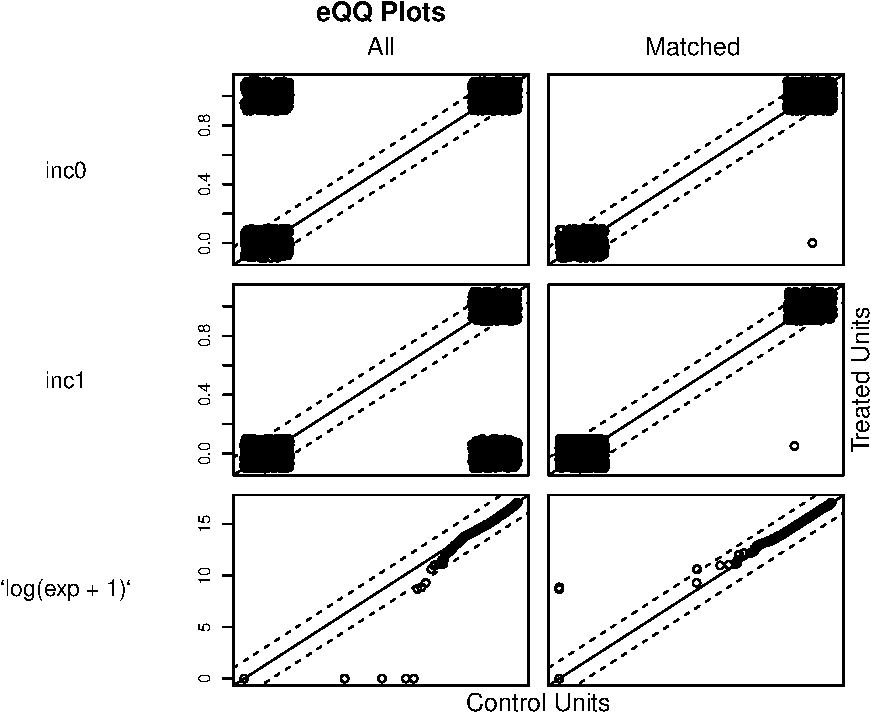
\includegraphics[width = 0.48\textwidth]{figure/fig-balancing check-2.pdf}}}
  \hfill
  \subfigure{{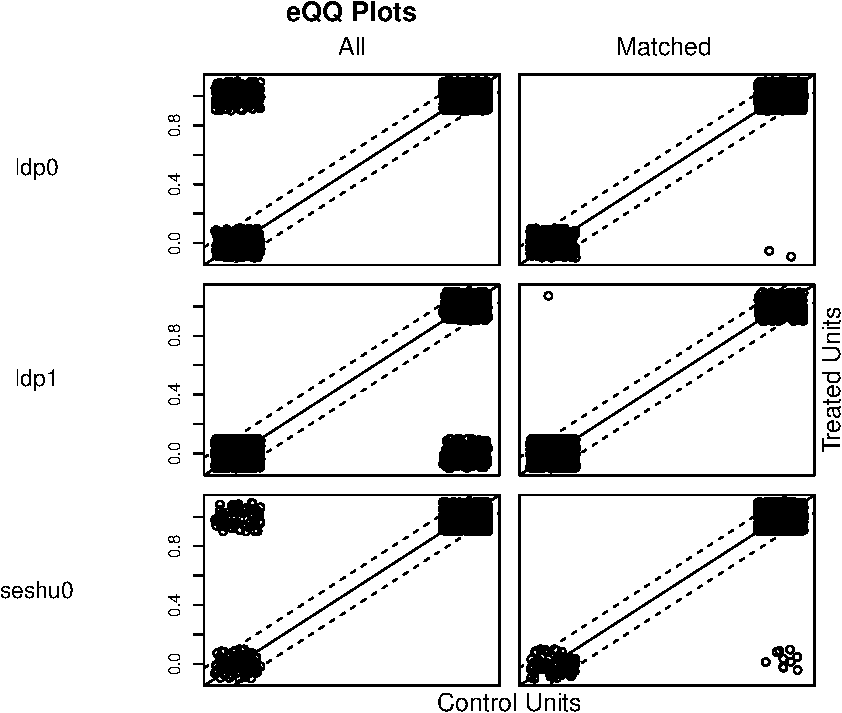
\includegraphics[width = 0.48\textwidth]{figure/fig-balancing check-3.pdf}}} \\
  \subfigure{{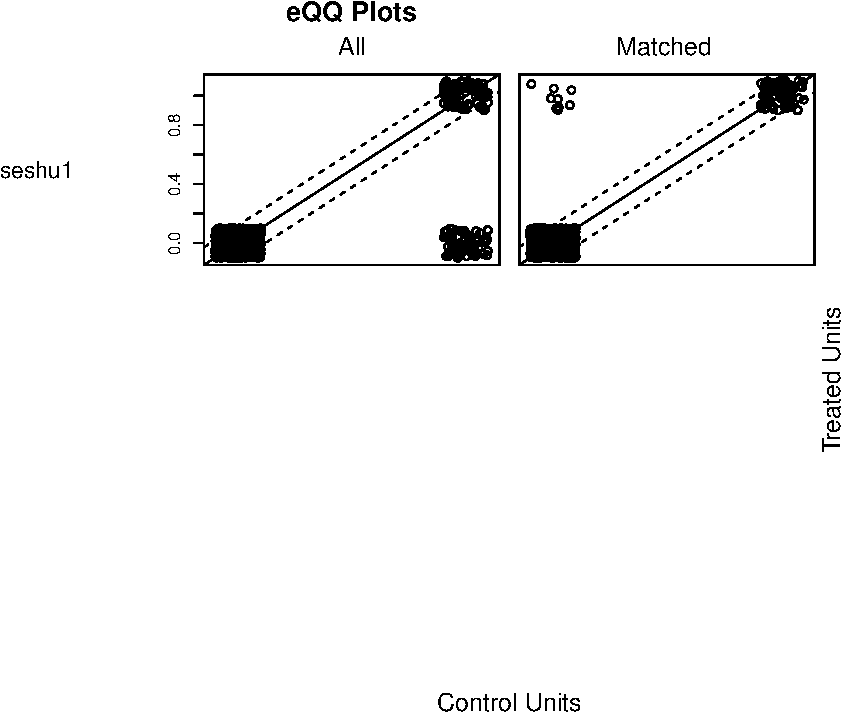
\includegraphics[width = 0.48\textwidth]{figure/fig-balancing check-4.pdf}}}
  \caption{Empirical Q-Q plots}
  \label{qq}
\end{figure}

One notable thing about this paper is that it incorporates multiple imputation and matching in its empirical analyses. Conforming to \citet{leyrat2019propensity}, I first create imputed data sets, calculate propensity scores in each of them, estimate parametric models for each of them, and then combine estimates to obtain aggregated values. 

\section{Analysis} \label{ch5}

This chapter consists of two sections that describe the estimation results of 1. multiply-imputed data sets and 2. multiply imputed, matched data sets. 

\subsection{Linear model} \label{ch5.1}

Table \ref{table:linear} shows the results of estimating multiply-imputed data sets \footnotemark{}. Models 1 - 5 correspond to those in the section \ref{ch4.2}. The estimates from each data set are combined according to Rubin's rules \citep{schafer1998multiple}. The number of observations in the table is the average of all data sets. 

% on Texreg
\footnotetext{Regression tables in this paper are compiled using R's \texttt{texreg} package \citep{leifeld2013texreg}. }

% regression table

\begin{table}[h]
\begin{center}
\scalebox{0.9}{
\begin{tabular}{l D{.}{.}{4.6} D{.}{.}{4.6} D{.}{.}{4.6} D{.}{.}{4.6} D{.}{.}{4.6}}
\toprule
 & \multicolumn{1}{c}{Model 1} & \multicolumn{1}{c}{Model 2} & \multicolumn{1}{c}{Model 3} & \multicolumn{1}{c}{Model 4} & \multicolumn{1}{c}{Model 5} \\
\midrule
(Intercept)               & 14.217^{***}           & 6.222^{***}            & 1.074                  &                         &                         \\
                          & (0.904)                & (0.969)                & (3.056)                &                         &                         \\
Age                       & 0.252^{***}            & -0.069^{***}           & 0.018                  & -0.092^{***}            & -0.068                  \\
                          & (0.018)                & (0.012)                & (0.055)                & (0.013)                 & (0.062)                 \\
Incumbency                &                        & 17.429^{***}           & 13.880^{***}           & 17.226^{***}            & 13.470^{***}            \\
                          &                        & (0.341)                & (1.525)                & (0.332)                 & (1.506)                 \\
Expenditure: log          &                        & 0.920^{***}            & 1.335^{***}            & 1.073^{***}             & 1.302^{***}             \\
                          &                        & (0.049)                & (0.212)                & (0.050)                 & (0.216)                 \\
LDP                       &                        & 15.325^{***}           & 27.308^{***}           & 14.698^{***}            & 30.689^{***}            \\
                          &                        & (0.346)                & (2.503)                & (0.355)                 & (3.223)                 \\
Inheritance               &                        & 6.702^{***}            & 7.362                  & 7.079^{***}             & 6.475                   \\
                          &                        & (0.539)                & (6.041)                & (0.572)                 & (6.621)                 \\
Age * Incumbency          &                        &                        & 0.069^{*}              &                         & 0.072^{*}               \\
                          &                        &                        & (0.028)                &                         & (0.028)                 \\
Age * Expenditure         &                        &                        & -0.007                 &                         & -0.003                  \\
                          &                        &                        & (0.004)                &                         & (0.004)                 \\
Expenditure * LDP         &                        &                        & -0.756^{***}           &                         & -1.010^{***}            \\
                          &                        &                        & (0.157)                &                         & (0.201)                 \\
Expenditure * Inheritance &                        &                        & -0.040                 &                         & 0.038                   \\
                          &                        &                        & (0.372)                &                         & (0.410)                 \\
\midrule
Fixed Effects             & \multicolumn{1}{c}{No} & \multicolumn{1}{c}{No} & \multicolumn{1}{c}{No} & \multicolumn{1}{c}{Yes} & \multicolumn{1}{c}{Yes} \\
Num. obs.                 & 8976.0               & 8976.0               & 8976.0               & 8976.0                & 8976.0                \\
\bottomrule
\multicolumn{6}{l}{\scriptsize{$^{***}p<0.001$; $^{**}p<0.01$; $^{*}p<0.05$}}
\end{tabular}
}
\caption{Linear Models}
\label{table:linearCh4}
\end{center}
\end{table}



What can we say about the age effect in the election? Model 1 in the first column represents the result of univariate regression. Claiming the age effect seems feasible: all other things being equal, a one-year older candidate is estimated to obtain a 0.25 \% larger vote share. 10 years of age difference could thus lead to 2.5 \% of gap. However, other models disagree. The inclusion of covariates overturns this positive significant age effect. Model 2, with four confounders, implies the negative, significant age effect. One year of age difference is related to a more moderate 0.07 \% change in vote share. 

What if we assume heterogeneous effects? The model assumes that the age and expenditure effects on candidates' performances are non-linear. The former effect is supposed to depend on candidates' incumbency status and the amount of campaign spending, and the latter effect is presumed to correlate with their affiliation and inherited political resources. Now, the age effect in the second row is non-significant. 

Furthermore, Models 4 and 5 add two-way fixed effects to Models 2 and 3 to account for the district- and year-level factors. Considering geographical and temporal elements does not change the interpretation a lot. These two models each signify a negative and non-significant age effect. Variables that show a significant effect in the models without fixed effects are estimated to have one in the same direction. Null results are also stable among these two sets of models. 

In addition to the disagreement with the hypothesis \ref{hyp:first}, the estimation points to the factors hidden under the veil of the superficial age effect. Mainly, incumbency, a greater amount of campaign expenditure, and affiliation with the LDP all work in favor of candidates. Models 2 and 4 also designate the advantage gained by inheriting electoral bases from relatives.

These estimation results support the hypothesis \ref{hyp:second}: the absence of the age effect in the lower house election. While the most simple model emits a significant positive relationship between candidates' age and their electoral performances, more complex models reverse or, at best, nullify this result. Overall, candidates' age appears not to matter significantly in the election. Young candidates' predicament may not originate from their age but from their other attributes. 

\subsection{Matching} \label{ch5.2}

Table \ref{table:matched} shows the results of estimating multiply-imputed, matched data sets. As in the table \ref{table:linear}, models 1 - 5 correspond to those in section \ref{ch4.2}. In the estimation process, missing data are first imputed. Then, propensity scores based on the hypothetical treatment variable are calculated for each imputed data. Data are matched via the method specified in the section \ref{ch4.3}, and parametric models are estimated for each matched data set. Finally, the resulting parameters are aggregated according to Rubin's rules. 

% regression table

\begin{table}[h]
\begin{center}
\begin{threeparttable}
\begin{tabular}{l D{.}{.}{4.4} D{.}{.}{4.4} D{.}{.}{4.4} D{.}{.}{4.4} D{.}{.}{4.4}}
\toprule
 & \multicolumn{1}{c}{Model 1} & \multicolumn{1}{c}{Model 2} & \multicolumn{1}{c}{Model 3} & \multicolumn{1}{c}{Model 4} & \multicolumn{1}{c}{Model 5} \\
\midrule
(Intercept)               & 23.699                 & -6.010                 & -43.899                &                         &                         \\
                          & (0.349)                & (1.978)                & (8.675)                &                         &                         \\
Treatment                 & -0.538                 & 1.600                  & 44.510                 & 1.801                   & 48.909                  \\
                          & (0.554)                & (0.413)                & (8.603)                & (0.425)                 & (4.069)                 \\
Incumbency                &                        & 15.961                 & 14.844                 & 15.321                  & 14.132                  \\
                          &                        & (1.978)                & (8.675)                & (0.563)                 & (0.681)                 \\
Expenditure: log          &                        & 1.488                  & 4.001                  & 1.639                   & 4.449                   \\
                          &                        & (0.413)                & (8.603)                & (0.425)                 & (4.069)                 \\
LDP                       &                        & 16.266                 & 54.899                 & 16.046                  & 62.455                  \\
                          &                        & (1.978)                & (8.675)                & (0.563)                 & (0.681)                 \\
Inheritance               &                        & 8.165                  & 43.080                 & 8.370                   & 40.150                  \\
                          &                        & (0.413)                & (8.603)                & (0.425)                 & (4.069)                 \\
Treatment * Incumbency    &                        &                        & 1.103                  &                         & 0.572                   \\
                          &                        &                        & (8.675)                &                         & (0.681)                 \\
Treatment * Expenditure   &                        &                        & -2.848                 &                         & -3.119                  \\
                          &                        &                        & (8.603)                &                         & (4.069)                 \\
Expenditure * LDP         &                        &                        & -2.489                 &                         & -2.989                  \\
                          &                        &                        & (8.675)                &                         & (0.681)                 \\
Expenditure * Inheritance &                        &                        & -2.160                 &                         & -1.964                  \\
                          &                        &                        & (8.603)                &                         & (4.069)                 \\
\midrule
Fixed Effects             & \multicolumn{1}{c}{No} & \multicolumn{1}{c}{No} & \multicolumn{1}{c}{No} & \multicolumn{1}{c}{Yes} & \multicolumn{1}{c}{Yes} \\
Num. obs.                 & 4725.0               & 4725.0              & 4725.0               & 4725.0                & 4725.0               \\
\bottomrule
\end{tabular}
\begin{tablenotes}[flushleft]
\scriptsize{
\item Treatment is to be younger than 
      (Average age of candidates in a particular election) - 
      (Standard deviation of candidates' age in that election).
}
\end{tablenotes}
\end{threeparttable}
\caption{Linear Models: Post-Matching Analysis}
\label{table:matched}
\end{center}
\end{table}



Results from the post-matching analysis are in a similar direction to those from the previous section. Multivariate models used in this part of the analysis suggest a positive, significant treatment effect. That is, being relatively young in a particular election benefits candidates. The coefficients of other variables are similar to those in the table \ref{table:linear}. Incumbency, amount of campaign spending, affiliation with the LDP, and inherited electoral resources are all positively correlated with candidates' performances in the election. Similarly, including two-way fixed effects does not make a significant difference in terms of significance and sign of the values. 

In sum, regardless of matching, estimation results are consistent with the hypothesis \ref{hyp:second}. The age effect in the election seems non-existent, and young candidates' other attributes are likely to be responsible for the uphills they face. 

\section{Discussion} \label{ch6}

This chapter outlines the results of this paper, summarizes its contributions, and discusses its limitations. Besides, it proposes the future direction of research working on youth under-representation in Japan. 

\subsection{Results} \label{ch6.1}

As the previous chapter illustrates, this paper's estimation results endorse the hypothesis \ref{hyp:second}: that is, although younger candidates are more likely to be ruled out of electoral races, they seem to be as competent as those of other ages, all things being equal. Instead, contributing to young candidates' plight in the election is that they are, on average, less endowed with various electoral resources, such as incumbency advantage, an affluent budget, affiliation with the dominant party, and inherited supports derived from kinship. 

Furthermore, some models not only nullify the age effect hypothesis but also turn it around. Voters do not dismiss young candidates. Rather, they might be favorable toward such novitiates. In other words, in a choice among candidates of different ages and the same attributes, the youngest candidate could obtain the largest vote share. 

These findings are in line with previous research in this area. In experimental settings with hypothetical candidates, scholars have found that participants do not avoid young candidates and rather prefer them on average \citep{horiuchi2020identifying, eshima2022just, mcclean2022too}. They are also consistent with the findings from research in different contexts \citep{stockemer2023young}. Together with these precedent works, it is reasonable to posit that there is no age effect in the Japanese lower house election. 

\subsection{Contributions} \label{ch6.2}

This paper's contributions are threefold. Firstly, it analyzes candidate-level data to obtain implications about youth under-representation. Previous research's focus is on higher, macro-level institutional factors, such as electoral systems. In contrast, this paper focuses on micro-level factors on the candidates' side and discerns, if not causally, factors preventing more youth from entering parliament. 

Secondly, this paper fills the gap in the literature on youth under-representation in Japan by providing an observational study on the age effect in the election. As stated multiple times in the preceding chapters, researchers have employed survey experiments to examine the voter perception of young candidates, which renounces and reverts the hypothesis of such an effect. These findings are valid for hypothetical candidate profiles and have not been tested with the actual candidates, at least in Japan. I exploit an comprehensive data set of the Japanese lower house candidates to assess the validity of those findings. The result is compatible with the previous research, suggesting the absence of the age effect and indicating the inverse version of it. 

Thirdly, this paper casts light on variables behind the spurious correlation between candidates' age and their electoral performances. Empirical analyses demonstrate that young candidates' lack of favorable attributes, such as incumbency status, affluent campaign spending, affiliation with the dominant party, and political dynasty, is correlated with their apparent disadvantage in the election. This suggestion shifts our attention upstream to the candidate selection process: youth under-representation could be founded in the pre-election stage. As research on the representation of other politically disadvantaged groups implies, the current situation might ameliorate once enough young candidates are provided into the election stage. 

\subsection{Limitations} \label{ch6.3}

While contributing to the literature from different aspects, this paper has some limitations and weaknesses. Firstly, this paper does not intend to make causal claims. Using observational data necessitates robust research designs to ``make the move from correlation to causation persuasive" \citep{sekhon2009opiates}, such as difference-in-difference and regression discontinuity, while this paper employs no such designs. Thus, its results should be accepted with a grain of salt: they indicate the absence of the age effect, but it could only be a correlation. 

Secondly, estimates in the empirical analysis might not possess ideal statistical properties, such as unbiasedness and consistency. This is due to the potential violation of assumptions. Most importantly, the random sampling assumption does not hold, as actual candidates in the pool of potential candidates self-select to run for the election. Also, vote shares (and the numbers of votes themselves) are mutually dependent on candidates in the same district-year. While including two-way fixed effects could amend the latter problem, the former undoubtedly persists.

Further, we cannot be sure about the absence of omitted variable bias. Whereas parametric models control several variables to account for the bias, the possibility is ultimately tenacious that there are excluded or unobserved variables that confound the relationship of interest. Altogether, these problems limit the reliability of estimates of the empirical analysis and the results' generalizability. Extrapolation of these results requires caution. 

Last but less importantly, the data cleaning process might be potentially problematic. Specifically, I employed multiple imputation to complete the data set, but the underlying assumption that missing variables are MAR might not be feasible. This data treatment could lead to a further bias in the estimates, should they be NMAR. 

\subsection{Future direction} \label{ch6.4}

How can we advance from now on? Broadly speaking, the main focus of research on youth under-representation, whether in the context of Japan or more generally, would be on the supply side arguments featuring pre-election stages. This paper consolidates the theory that young candidates' age is not disadvantageous to their performances. Given that few young candidates are running for the election, as chapter \ref{ch2} showed, our next question could be, for example, ``What prevents young people from running for the election?". As \citet{lawless2010still} points out, it takes candidates for disadvantaged groups to be represented in parliament. If we are concerned about the youth under-representation or its potential consequence in terms of policy, it would be natural to speculate on the causes of the deficiency of young candidates. 

\section{Conclusion}

Accounting for a good part of the population, the youth in Japan are under-represented in political decision-making. There are small numbers of young parliamentarians or candidates, but comparing the two reveals that young candidates are more likely to be eliminated in the election. The question is, ``Does the age itself matter?". 

This paper tries to answer this question using comprehensive data from candidates who ran for the Japanese lower house election. Previous research has repudiated the age effect in the election on the ground that voters are, on average, more favorable toward young candidates when they face a choice between hypothetical candidates. An observational study of the actual candidates' data delivers evidence from another perspective. 

The results are in line with the existing inquiries. Data show that while young candidates suffer in the election for their age, this relationship is meretricious, induced by their lack of advantageous properties like incumbency, financial resources, strong party affiliation, and inherited electoral bases. All other things being equal, young candidates seem to be as competent as other age groups. Jennifer Lawless and Richard Fox once wrote on female under-representation: "When women become candidates and make it to Election Day, they perform as well as men"(\citet{lawless2010still}, 174). The same would apply to the youth. 

Where should we head now? Interested in the source of the youth under-representation, we turn our eyes toward the upstream of the river: to the dam controlling the flow of water (i.e., party gatekeepers) and the source (i.e., the pool of potential candidates). We still lack young candidates, and further investigations should focus on the process preceding the election.

\newpage

% Reference
\bibliography{../Literature.bib}
\bibliographystyle{apalike}

\end{document}
